%% Test ❤ 111000101000100010011110 1100000010101111

\documentclass{article}

\usepackage{amsmath}
\usepackage{amsfonts}
\usepackage{cjhebrew}
\usepackage{parskip}
\usepackage[hidelinks]{hyperref}
\usepackage{xcolor}
\usepackage{graphicx}

\renewcommand{\contentsname}{Tabla de contenidos}
\renewcommand{\refname}{Referencias}

\title{\vspace{-1.7cm}\textbf{Codificación UTF-8}}
\author{Diego José Abengózar Vilar, Julio César Castro López}
\date{26/3/2021}

\begin{document}

\maketitle
\tableofcontents

\section{Contexto histórico}

En los años 60 y 70, cuando el uso de los ordenadores no era tan universal como ahora, se utilizaban unos pocos caracteres: letras del alfabeto romano sin tildes. Eran tan pocos símbolos que se podían codificar perfectamente en 7 bits, en un código llamado ASCII.

\begin{figure}[h]
  \centering
  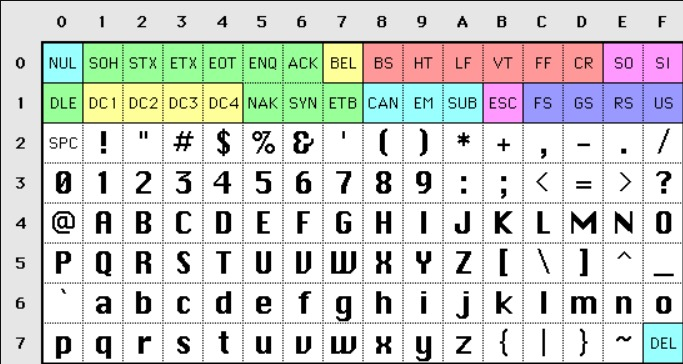
\includegraphics[scale=0.65]{ascii.jpeg}
  \caption{Tabla ASCII}
\end{figure}

De hecho, como sobraba 1 bit para llegar a la unidad tradicional de 1 byte, los vendedores de PC de la época empezaron a darle uso a este último bit para permitir, por ejemplo, el uso de letras con tilde en el caso de muchos países europeos, o carácteres hebreos en los ordenadores vendidos en Israel. En muchos PCs europeos el caracter 130 se visualizaba como `é'' mientras que en los ordenadores de Israel se visualizaba como `\cjRL{g}''. Esto tenía el problema de que, si se enviaba un documento codificado en un ordenador con una cierta especificación a otro con una especificación distinta, se producían traducciones erróneas. El problema era aún mayor en países asiáticos, ya que el número de símbolos de sus lenguajes no cabían en 8 bits.

Con la llegada de Internet, esta codificación era insuficiente y en 1991 surgió \textit{Unicode} para includir todos los caracteres de cualquier sistema de escritura del planeta. Cada símbolo está asociado a un punto de código (\textit{code point}), que se suele escribir de la forma $U+XXXX$, donde $XXXX$ son dígitos hexadecimales, y que luego se trasladará a un cierto número de bytes. Al principio se decidió utilizar 2 bytes para cada punto de código, pero pronto se dieron cuenta de que, en muchas ocasiones, las cadenas estaban llenas de ceros pues sobraba mucho espacio para los caracteres de uso común. Además, al utilizar 2 bytes podía haber problemas para determinar el orden de los mismos (\textit{endianness}).

Para solucionar estos problemas se inventó UTF-8, que utiliza un número variable de bloques de 1 byte.

\section{Desarrollo Teórico}

\subsection{Especificación}

UTF-8 es una codificación de tamaño variable: codifica la información utilizando entre 1 y 4 octetos. Está pensado además para ser una correspondencia perfecta con el código ASCII, es decir, un texto codificado con ASCII tendría la misma codificación en UTF-8 y no hay ningún otro texto codificado en UTF-8 que pudiera ser interpretado como ASCII.

Los caracteres Unicode se designan con la notación $U+XXXX$, donde $XXXX$ es una cadena de entre 4 y 6 dígitos hexadecimales.

El número de octetos que se emplean dependen del caracter a codificar:

\begin{itemize}
  \item Los caracteres con números desde $U+0000$ hasta $U+007F$ se codifican con un octeto de bits que va desde el valor $0x00$ hasta $0x7F$ (0 - 127 en decimal). Nótese que con 7 bits se pueden codificar 128 valores ($2^7 = 128$), por lo que la cifra más significativa del octeto toma valor 0 y con las otras siete se codifica el valor correspondiente. Esto es una correspondencia exacta con ASCII.
  \item Los caracteres con números desde $U+0080$ hasta $U+07FF$ se codifican con dos octetos (128 - 2047 en decimal). Los primeros tres bits del primer octeto son $110$ y los dos primeros bits del segundo octecto son $10$. Con los 11 bits restantes basta para codificar el valor correspondiente.
  \item Los caracteres con números desde $U+0800$ hasta $U+FFFF$ se codifican con tres octetos (2048 - 65535 en decimal). Los primeros cuatro bits del primer octeto son $1110$ y los dos primeros bits de los octetos siguientes son $10$. Con los 16 bits restantes se codifica el valor correspondiente.
  \item Los caracteres con números desde $U+10000$ hasta $U+10FFFF$ se codifican con tres octetos (65536 - 1114111 en decimal). Los primeros cinco bits del primer octeto son $11110$ y los dos primeros bits de los octetos siguientes son $10$. Con los 21 bits restantes se codifica el valor correspondiente.
\end{itemize}

En la siguiente tabla presentamos un resumen de los disintos formatos.

\begin{table}[h!]
  \centering
  \begin{tabular}{|l||l|}
    \hline
    Rango de números       & Tipo de codificación                        \\ \hline \hline
    $0x00$ - $0x7F$        & $0xxxxxxx$                                  \\ \hline
    $0x80$ - $0x7FF$       & $110xxxxx$ $10xxxxxx$                       \\ \hline
    $0x800$ - $0xFFFF$     & $1110xxxx$ $10xxxxxx$ $10xxxxxx$            \\ \hline
    $0x10000$ - $0x10FFFF$ & $11110xxx$ $10xxxxxx$ $10xxxxxx$ $10xxxxxx$ \\ \hline
  \end{tabular}
\end{table}

Como vemos, el primer octeto empieza con tantos $1$ como número de octetos tiene la codificación (salvo cuando solo hay uno), y los posteriores octetos empiezan con $10$. Se codifican todos los valores del rango $0x0$ hasta $0x10FFFF$, lo que da cabida a más de un millón de caracteres.

\subsubsection{Codificación}

\begin{enumerate}
  \item Se determina el número de octetos a partir del número de caracter.
  \item Se colocan los bits más significativos según la tabla anterior.
  \item Para rellenar el resto de bits se toma el bit menos signifcativo del número de caracter a codificar y se coloca en la posición menos significativa del último de los octetos. A continuación se toma el segundo bit menos significativo del número de caracter a codificar y se coloca en la segunda posición menos significativa del último de los octetos. Se sigue con este procedimiento hasta rellenar todos los bits, pasando al octeto siguiente cuando corresponda y completando con $0$ si es necesario.
\end{enumerate}

\paragraph\*{Ejemplo}

Si queremos codificar $U+2764$, primero observamos que $0x0800 < 0x2764 < 0xFFFF$, y por tanto tiene 3 octetos:
\[1110xxxx \; 10xxxxxx \; 10xxxxxx\]

$0x2764$ en binario es ${\color{green}0010} {\color{blue}0111 01}{\color{red}10 0100}$ y colocamos los bits menos significativos en la posiciones menos significativas:
\[1110\mathbf{{\color{green}0010}} \; 10\mathbf{{\color{blue}0111 01}} \; 10\mathbf{{\color{red}10 0100}}\]

\subsubsection{Decodificación}

\begin{enumerate}
  \item Se inicializa un número binario con todos los bits a 0. Nótese que no hacen falta más de 21 bits.
  \item Se determina el número de octetos y qué posiciones contienen la información del caracter codificado.
  \item Se colocan los bits desde la posición menos significativa del último octeto hasta la más sigificativa del primer octeto en nuestro número binario en ese mismo orden, es decir, empezando por los bits menos significativos.
\end{enumerate}

\paragraph\*{Ejemplo}

Si nos dan $111000101000100010011110$, determinamos que tiene 3 bloques ya que empieza por $111$ e identificamos los bits que codifican la información:
\[1110\mathbf{0010} \; 10\mathbf{001000} \; 10\mathbf{011110}\]

Nos queda el número $0010001000011110$, lo pasamos a hexadecimal:
\[0010 \; 0010 \; 0001 \; 1110 = 0x221E\]

Por tanto el caracter UTF-8 codificado es $U+221E$.

Supongamos ahora que nos dan la secuencia $0xC0AF = 1100000010101111$. Si la decodificamos siguiendo el procedimiento anterior:
\[110\mathbf{00000} \; 10\mathbf{101111}\]
\[000 \; 0010 \; 1111 = 0x02F = U+002F\]

Sin embargo, si nos fijamos bien, el caracter $U+002F$ $(0x{\color{blue}2}{\color{red}F} = {\color{blue}10}{\color{red}1111})$ lo habríamos codificado de la siguiente manera:
\[0xxxxxxx\]
\[00{\color{blue}10}{\color{red}1111} = 0x2F\]

¿Hay acaso dos secuencias tales que al decodificarlas dan el mismo caracter? No, la implementación solo debe tomar como secuencia válida la más pequeña que codifica el caracter. La secuencia $0xC0AF$ del ejemplo es conocida como una \textit{overlong sequence} y no es aceptada como válida por la especificación.
El estándar también prohibe la codificación de los caracteres entre $U+D800$ y $U+DFFF$.

Otra consideración a hacer es el caracter $U+FEFF$, conocido como \textit{Byte Order Mark}. Si se se encuentra al comienzo, sirve para indicar el orden de los bytes (\textit{endianness}). Esto es relevante para otras codificaciones Unicode que utilizan bloques de 16 o 32 bits, aunque no tiene mayor importancia en el caso de UTF-8.

\section{Desarrollo Informático}
\href{https://codificacion-criptografia.gitlab.io/utf/}{\textit{https://codificacion-criptografia.gitlab.io/utf/}}

\subsection{Implementación}
No sé exactamente que deberíamos poner aquí.ddddddddddd

\subsection{Visualización}
hola buenas

\section{Aportaciones personales y conclusiones}
Este es el título de la sección que propone el profesor. A saber qué poner xD.

\addcontentsline{toc}{section}{Referencias}
\begin{thebibliography}{9}

  \bibitem{utf8}
  F. Yergeau,
  \href{https://tools.ietf.org/html/rfc3629}{\textit{RFC 3629 - UTF-8, un formato de transformación de ISO 10646}},
  Internet Society, 2003

  \bibitem{historia}
  Joel Spolsky,
  \href{https://www.joelonsoftware.com/2003/10/08/the-absolute-minimum-every-software-developer-absolutely-positively-must-know-about-unicode-and-character-sets-no-excuses/}{\textit{The Absolute Minimum Every Software Developer Absolutely, Positively Must Know About Unicode and Character Sets (No Excuses!)}},
  2003

\end{thebibliography}

\end{document}
